\documentclass[letterpaper, 12pt]{article}
\usepackage[top=2cm,bottom=1cm,left=0.75in,right=0.75in,headheight=17pt, % as per the warning by fancyhdr
includehead,includefoot,
heightrounded, % to avoid spurious underfull messages
]{geometry}
\addtolength{\topmargin}{-.25in}
\usepackage{fancyhdr}
\pagestyle{fancy}
\usepackage{graphicx}
\usepackage{lastpage}
\usepackage{gensymb}
\usepackage[american]{circuitikz}

\begin{document}
\fancyhead[l]{	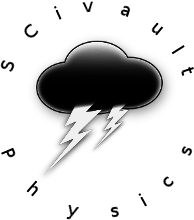
\includegraphics[height=1.2cm]{../Logo/sp.png} Name:}
\fancyhead[r]{REFERENCE MATERIAL}
\cfoot{\thepage\ of \pageref{LastPage}}
	


\begin{center}Things to Memorize: Magnetic Forces and Fields
\end{center}
\vspace{-.6cm}
\subsubsection*{Cross Products and the First Right Hand Rule}
\begin{itemize}
	\item To find the magnitude of a cross product like $ \vec{A} \times \vec{B}$, multiply $|A| \cdot |B| \cdot \sin(\theta) $ 
	\item To find the direction of the resultant vector use the \textbf{First Right Hand Rule}:
	\begin{enumerate}
		\item Point your index finger in the direction of the first vector ($\vec{A}$).
		\item Bend your middle finger $90 \degree $ and rotate your arm to point it in the direction of the second vector ($\vec{B}$).
		\item Your thumb will point in the direction of the resultant vector.
		
		\textit{Note: The resultant vector is always perpendicular to both of the original vectors.}
	\end{enumerate}
\end{itemize}
\vspace{-.5cm}

\subsubsection*{Magnetic Force}
\begin{itemize}
	\item On a charged particle.
		\begin{itemize}
			\item Magnetic fields exert forces on \textbf{moving, charged} particles.
			\item Charged particles tend to move in a \textbf{circle} or \textbf{helix (spiral)} in a magnetic field.
			\item Particles do not feel a force when they travel parallel or antiparallel to the magnetic field. 
			\item The Magentic Force on a particle is often canceled by an electrostatic force.  In this case, particles of only a specific velocity can move through the area without colliding with the walls of the device.
			
		\end{itemize}
	\item On a wire carrying current.
		\begin{itemize}
			\item A wire will not feel a force if it carries current parallel or antiparallel to the magnetic field.
			\item Even thought the formula is $ F_b = I \vec{\ell} \times \vec{B} $, the direction of the first vector ($\vec{\ell}$) is in the direction of the current. 
		\end{itemize}
	
\end{itemize}

\subsubsection*{Magnetic Fields}
\vspace{-.3cm}
\begin{itemize}
	\item Moving charges generate magnetic fields. 
	\item The direction of the magnetic field generated by a current-carrying wire is given by the \textbf{Second Right Hand Rule}: 
	\begin{enumerate}
		\item Point your thumb in the direction of the current flow.  
		\item Pretend to grab the wire with your hand.  
		\item The magnetic field will wrap around the wire in the direction your fingers point.
	\end{enumerate}
	\item The direction of the magnetic field generated by a coil or a loop of wire is given by the \textbf{Third Right Hand Rule}:
	\begin{enumerate}
		\item Coil your fingers in the same direction as current flows.  
		\item Your thumb points in the direction of the magnetic field. 
	\end{enumerate}
\end{itemize}



\end{document}
